\chapter{Introduction}

You know the problem, when you are on a sightseeing-trip in a city and want to take a picture of some
building or just a nice place. But there are annoying persons moving around in front
of the object!

So why don't you use our MOPET Software?
All you need is a series of at least 5 pictures of the object. The software 
detects all moving persons and objects and removes them.

\begin{figure}[h!]
 \centering
 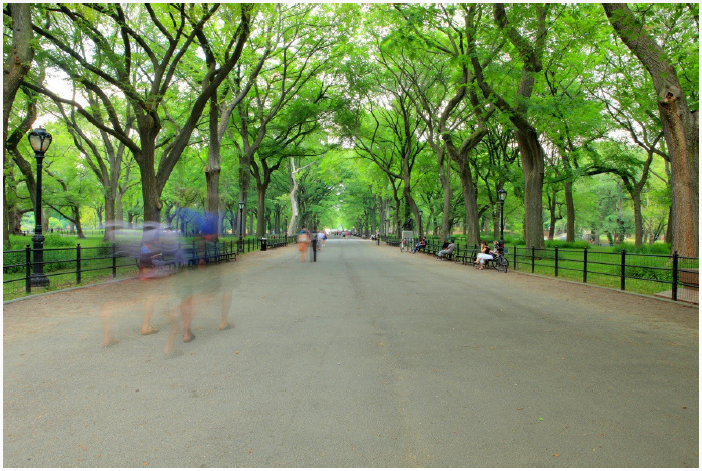
\includegraphics[width=\textwidth]{./pics/intro.png}
 % intro.png: 702x471 pixel, 72dpi, 24.76x16.61 cm, bb=0 0 702 471
 \caption{The goal of our project: remove moving foreground objects in a scene.
 Source: [http://www.digital-photography-school.com]}
 \label{fig:intro}
\end{figure}



\chapter{Methods}

Unfortunately, we did not find any papers or other literature to this topic. Most of the methods for estimating
background are using a video stream as input and estimate the optical flow.
We decided to use a series of images,
because the quality of a single picture is much better than the quality of a frame in a video.
The major difference between a video stream and a series of pictures is the time between two frames.
In a video it is possible to estimate the optical flow, because there is not too much movement in the scene.
When you have a series of images from a continuous shooting it is very difficult to estimate the optical flow, because the time between
two images is too long and may not find any correspondences in the image.

Therefore, we came up with our own idea.

\section{Registration of images}

We don't assume that the series of pictures are taken using a tripod.
Because of small movements of the camera during a continuous shooting, the image section may move
around.
Therefore, we need to align the images with the following steps.

\begin{itemize}
 \item Applying a feature-detector to all images and calculating feature descriptors.
  As a feature-detector we used FAST and for the descriptor SURF.
 \item the feature detector FAST detects up, to 100000 keypoints in our input images.
 From this set of keypoints we selected a random subset of 10000 keypoints.
 \item The feature-descriptors of all images are matched to the features of the first image.
 \item RANSAC is used to estimate a homography, which is robust against outliers due to moving foreground.
 \item All images are then warped, to the position of the first image.
\end{itemize}



\section{Foreground/Background Classification}

To classify between moving Foreground and static Background, we developed our own method called
``Minimum Variance Classifier''.

We are using the following assumptions to distinguish between foreground and background.

\begin{itemize}
 \item Moving Foreground leads to different pixel values with a large variation.
 \item Static background should lead to very similar pixel values.
 \item Therefore, the variance of the background pixels should be lower than the variance of the foreground.
\end{itemize}
 
First, we perform a gaussian filtering to reduce the influence of noise. For this purpose a
gaussian kernel with sigma of around 3 to 6, showed the best results.
A too small sigma would not sufficiently suppress noise,
and a too large sigma would not lead to a accurate estimation of foreground and background.

Now we iterate through all (x,y) positions of the image and perform the following steps:

\begin{enumerate}
 \item Sort the different pixel values $I(x,y,t)$ at position (x,y) according to their gray values.
 $x$ and $y$ are the spatial coordinates in the image, while $t$ is the index of the $N$ images in the
 continuous shooting.
 \item From the sorted gray values $I_{sorted}(x,y,t)$ we now iterate through all
 possible connected groups of pixels and perform the following steps.
 \begin{enumerate}
  \item For each group of pixels $\Omega$ we caluclate a cost function $f(\Omega$)
  $$
  f(\Omega) = var\{R(\Omega)\} + var\{G(\Omega)\} + var\{B(\Omega)\} + \frac{\alpha}{length\{\Omega\}}
  $$
  $R(\Omega)$, $G(\Omega)$ and $B(\Omega)$ are the pixel values of the red, green and blue channel
  of the group. $length\{\Omega\}$ is the number of pixels in a group. $\alpha$ is a tuning parameter.
  
  The function leads to a large value if the variance of the pixel values is large, or if the 
  number of pixels in the group($length\{\Omega\}$) is small. The term $\frac{\alpha}{length\{\Omega\}}$
  is necessary, because in the next step we will perform a minimization of the function $f(\Omega)$.
  That minimization would always tend to prefer smaller group of pixels. 
  The reason for that is that the smaller groups of the sorted pixel values
  have more likely a smaller variance. A value $\alpha=200$ showed the best results in our experiments.
  \item If the value $f(\Omega)$ is smaller than the current minimum $f_{min}$ of the group $\Omega_{min}$:
  Set $f_{min}$ to $f(\Omega)$ and $\Omega_{min}$ to $\Omega$.
 \end{enumerate}
 \item From the previous steps we retrieved the group $\Omega_{min}$ with the smallest cost function
 $f_{min}$. Since this group minimizes the variance of the RGB channels this group will be classified as
 background.
 
 Therefore, set all pixel in the foregroundmask belonging to the group $\Omega_{min}$ to zero and
 all the other pixels at position (x,y) to 1.

\end{enumerate}

Finally, we applied the morphological operation closing to get a connected region
of our foreground objects and also the operation opening to remove single ``noise'' pixels, that have been
classified as foreground in the forground mask.


